\documentclass{article}
\usepackage[utf8]{inputenc}
\usepackage[spanish]{babel}
\usepackage{hyperref}
\usepackage{float}
\usepackage{graphicx}

\bibliographystyle{plain}

\title{Medida indirecta de la velocidad de la luz.}
\author{Ramón Merino Rojas}
\date{1 de Noviembre 2019}

\begin{document}

\maketitle

\begin{abstract}
Link al repositorio: \href{https://github.com/Ramonmr20/proyecto_final}{https://github.com/Ramonmr20/proyecto\_final}

En este artículo describiremos el proceso para poder medir la velocidad de la luz usando un microondas y una loncha de queso. Así mismo daremos los datos y conclusiones del experimento.

\textit{\textbf{Palabras clave:} velocidad de la luz, luz, radiacción electromagnética, relatividad, Einstein, microondas, queso, física, experimento.}
\end{abstract}


\tableofcontents

\section{Introduccion y estado del arte}
Desde que Einstein publicó su teoría de la relatividad especial en 1905, sabemos que la velocidad de la luz es constante. \cite{Paterna1971}

Esta constante es: $299 792 458 m/s$ pero, ¿cómo podemos medir esto?

Bien, antes de nada debemos aclarar que la luz no se trata solo de la luz visible, si no que el espectro electromagnético es mucho más amplio.


\begin{figure}
    \centering
    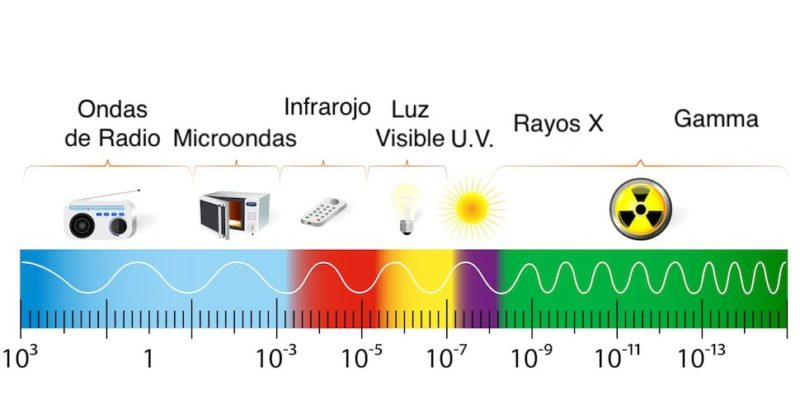
\includegraphics[width = 0.7\textwidth]{espectro}
    \caption{Representación gráfica del espectro electromagnético.}
    \label{fig:espectro}
\end{figure}

Como podemos apreciar en la figura \ref{fig:espectro} la luz es mucho más que lo vemos, se encuentra en los rayos x o gamma pasando por los microondas o las ondas de radio.

Usaremos los conceptos de frecuencia y longitud de onda de un microondas para poder medir la velocidad de la luz.
\section{Fundamento Teórico}

\section{Materiales y metodología}

\section{Resultados y conclusión}


\bibliography{bibli}
\end{document}
